\documentclass{tufte-handout}
\usepackage[letterpaper]{geometry}
\usepackage{fontspec}
\usepackage{termcal}
\usepackage{graphicx}


\geometry{
  left=1in, % left margin
  bottom=1in,
  top=1in,
  textwidth=25pc, % main text block
  marginparsep=2pc, % gutter between main text block and margin notes
  marginparwidth=12pc % width of margin notes
}

\makeatletter
\providecommand\tuftedate{}
\@ifpackageloaded{termcal}{%
  \renewcommand{\date}[1]{%
    \gdef\@date{#1}%
    \begingroup%
    % TODO store contents of \thanks command
    \renewcommand{\thanks}[1]{}% swallow \thanks contents
    \protected@xdef\tuftedate{#1}%
    \endgroup%
  }{%
    % Do nothing else, there's no need to redefine \date
  }
}
\makeatother
\defaultfontfeatures{Mapping=tex-text}

\renewcommand{\allcapsspacing}[1]{{\addfontfeature{LetterSpace=10.0}#1}}
\renewcommand{\smallcapsspacing}[1]{{\addfontfeature{LetterSpace=2.0}#1}}
\renewcommand{\textsc}[1]{\smallcapsspacing{\textsmallcaps{#1}}}
\renewcommand{\smallcaps}[1]{\smallcapsspacing{\scshape\MakeTextLowercase{#1}}}

\renewcommand{\calprintclass}{}

\title{2018 Syllabus for Biology 313: Plant Taxonomy}										% change each year
\author{Lecture: Tuesday/Thursday 8:00am--9:40am (251 ISC)}										% change per section
\date{Lab: Wednesday 1:20-5:20pm (251 ISC)}

\begin{document}
\maketitle

Instructor: Dr.~Althea A.~ArchMiller\marginnote{The schedules and policies associated with this course may be subject to revision or change as a consequence of changing circumstances or events. Reasonable notification will be provided to students prior to any major changes in course policies or procedures.}\\
Office: 220 Integrated Science Center\\
218.299.3793 (office) / 218.556.8053 (cell)\\
Email: aarchmil@cord.edu\\
Twitter: @aaarchmiller\\
Office Hours: Mon/Wed 10:30-11:00 \& T/Th 10:30-12:00


\begin{fullwidth}

\section{Course Description}

Identification, nomenclature, and classification of vascular plants. 

\subsection{Course Goals}

The primary objective of this course is to provide a basis for your understanding of plant taxonomy, which includes the identification, classification, and relationships of vascular plants and plant families. You will learn how to observe, describe, and draw the features of plants that make them identifiable and increase your knowledge of regional plant species. This class is also a field class, which means that you will get to enjoy spending 24+ hours outdoors in various climates and ecosystems!

\newthought{My learning outcomes for you} are being able to:

\begin{enumerate}
	\item Describe how plant families are related and classified
	\item Identify plants based on herbarium collections, dichotomous keys, and field guide books
	\item Hone your observation and drawing skills
	\item Maintain detailed and organized field notes
	\item Compare regional ecosystems and cultural features
	\item Communicate your scientific knowledge in meaningful and effective ways
\end{enumerate}

\newthought{Your personal learning outcomes} are being able to: 

\vspace{1.5cm}

\subsection{Required Material}

\begin{itemize}
	\item Murrell. \emph{Vascular Plant Taxonomy}. 2010. 6$^{th}$ Edition. Kendall Hunt.
	\item Chadde. \emph{Minnesota Flora: An Illustrated Guide to the Vascular Plants of Minnesota}. 2013. 
	\item Dedicated plant collection notebook such as ``Rite in the Rain'' or Moleskin. I recommend one with numbered pages and blank or faint horizontal lines. Sketchbooks also work well.
	\item 10x Hand Lens available for purchase from Joy Navratil in the Biology Department Office
	\item Various field guide books available in the lab classroom
	\item Supplemental material available on Moodle
\end{itemize}

%\section{Policies}

\subsection{Accommodations for Students with Disabilities}

In accordance with the Americans with Disabilities Act, Concordia College and your instructor are committed to making reasonable accommodations to assist individuals with documented disabilities to reach their academic potential. Such disabilities include, but are not limited to, learning or psychological disabilities, or impairments to health, hearing, sight, or mobility. If you believe you require accommodations for a disability that may impact your performance in this course, you must schedule an appointment with Disability Services to determine eligibility. Students are then responsible for giving instructors a letter from Disability Services indicating the type of accommodation to be provided; please note that accommodations will not be retroactive. The Disability Services office is in Academy 106, phone 218-299-3514; https://www.concordiacollege.edu/directories/offices-services/counseling-center-and-disabilityservices/disability/ 

\newthought{The best way to be successful in this class} is to take lots of hand-written notes in a lecture notebook and your field notebook, as appropriate. If you need accomodations for other learning techniques, please let me know as soon as possible. 

You may take photos of plants during fieldtrips, but *only* after first making complete field notes and drawings in your field notebook. \textbf{Please be respectful and turn your cell phones off during lecture.}

\subsection{Respect for Diversity}

It is my intent that students from diverse backgrounds and perspectives be well-served by this course, and that the diversity that students bring to this class be viewed as a resource. Please let me know ways to improve the effectiveness of the course for you, personally, or for other students or student groups. As a student in this class, you are required to treat other members of the class with respect and kindness. Disrespectful, rude, or exclusive behavior will not be tolerated.

\newthought{Official Diversity Statement:} Concordia College aspires to be a diverse community that affirms an abundance of identities, experiences, and perspectives in order to imagine, examine, and implement possibilities for individual and communal thriving. Critical thinking grounded in the liberal arts compels us to participate in intentional dialogue, careful self-reflection, and honest interactions about difference, power, and inequity. As responsible engagement in the world calls us to recognize worlds that are familiar or unfamiliar, visible or less visible, Concordia will act to increase and support diversity in all areas of campus life.

\end{fullwidth}

\section{Academic Integrity (from Student Handbook)}

\marginnote{I will not tolerate any instance of academic dishonesty, including cheating, plagiarism, falsification, facilitating others' violations, or impeding (see student handbook for definitions). }

%``Every member of our academic community is charged with the responsibility of maintaining an environment of integrity. Faculty bear special responsibilities in encouraging integrity. Their first responsibility is to function as models of academic integrity. 

``Students are responsible for maintaining and encouraging academic integrity at the college. We expect all students to act with integrity in the classroom and in completing and submitting assignments. Ultimately, students bear the responsibility of ensuring the integrity of their own work. Students are expected to meet at least the minimal requirements of each course with work of appropriate quality. 

\marginnote{Instances of academic dishonesty will result in either a failing grade for that activity or for the course, according to the perceived intent and extent of the instance(s) of academic dishonesty. All academic integrity violations will be reported to the Office of Academic Affairs.}

``At no time is cheating on examinations, quizzes, or assignments acceptable at Concordia. Students are also expected to exercise appropriate caution to avoid plagiarism on written assignments.''

\newpage


\section{Grades}

%Final grades will be based on the following:

%\emph{Note: This class will be heavily front-loaded because of the waning fall plant season. We will focus the first month on observing and identifying as many species as possible, so it is important to come to class prepared to learn and explore.}

\begin{margintable}
\begin{tabular}{rl}
Percentage & Grade \\
\hline 
$\ge94$ & A \\
90-93.9 & A- \\
87-89.9 & B+ \\
83-86.9 & B \\
80-82.9 & B- \\
77-79.9 & C+ \\
73-76.9 & C \\
70-72.9 & C- \\
67-69.9 & D+ \\
60-66.9 & D \\
$<60$ & F \\
\hline
\end{tabular}
\end{margintable}

\begin{table}
\begin{tabular}{l l l r r}
Category & Item & Date &  Pts & \% \\
\hline
Exams & & & & 35 \\
& Terminology Exam & Sept.~11 & 5\\
& Exam 1 & Oct.~9  & 10 \\
& Exam 2 & Nov.~20  & 10 \\
& Final Exam & Dec.~18 & 10 \\ 
\hline
Lab Exams & & & & 15\\
& Lab Exam 1 & Sept.~25  & 5 \\
& Lab Exam 2 & Oct.~18 & 5 \\
& Lab Exam 3 & Nov.~29  & 5 \\ 	
\hline
Plant Collection & & & & 30 \\
Notebook & Initial 15 spp. & Sept.~25 & 15 \\
& Second 10 spp. & Oct.~18 & 10 \\
& Final 5 spp. & Nov.~29 & 5 \\
\hline 
Other & & & & 20 \\
& Family Presentation & Dec.~5 & 15 \\
 & Participation &  & 5 \\
\hline
& & & Total 100 & 100\%
\end{tabular}
\end{table}

\begin{fullwidth}

\newthought{Exams} will test your understanding of plant taxonomy terminology, interrelatedness of plants and plant families, and cultural/economic properties of plants as covered in lectures. We will discuss important features and anatomy of approximately 100 plant families. 

\newthought{Lab Exams} will test your ability to identify plant species and plant families. Scientific names will need to be used and spelled correctly for full credit. Spelling errors and common names will be counted for partial credit. Specimens used in lab exams will be a combination of live plants, dried plants, twigs and/or fruit/seeds.

\newthought{The Plant Collection} will be a list of species provided in a table that will correspond with and be handed in with your field notebook.  For full credit, you will need to have scientific name and family (1pt), completed field notes (1pt), technical descriptions (1pt), and drawings (1pt) for each individual species you ``turn in'' for review. Species records can span multiple notebook pages (e.g., early season leaf drawing, later season twig drawing), but separate entries for the same species do not count as multple species. 

You will need to turn in 15 individual species at Lab Exam 1, an additional 10 at Lab Exam 2, and an additional 5 at Lab Exam 3 (see schedule and grade breakdown for specific dates). The final 30 species should cover at least 10 families.

This is an example of the table and of a full-credit notebook page. Note: drawings do not have to be perfect, but they do need to reflect specifics that would help in identifying that particular species. 

\begin{tabular}{lllllllll}
\hline
Plant & Family & \emph{Genus species} & Common name(s) & Type & Page(s) & Instructor Check & \\
\hline
1 & Lamiaceae & \emph{Monarda fistulosa} & wild bergamot & Forb & 13 & 9/25/2018: 4/4 \\
2 & Ulmaceae & \emph{Ulmus americana} & American elm & Tree & 11,20 & 9/25/2018: 3/4 \\
\vdots \\
\hline
\end{tabular}

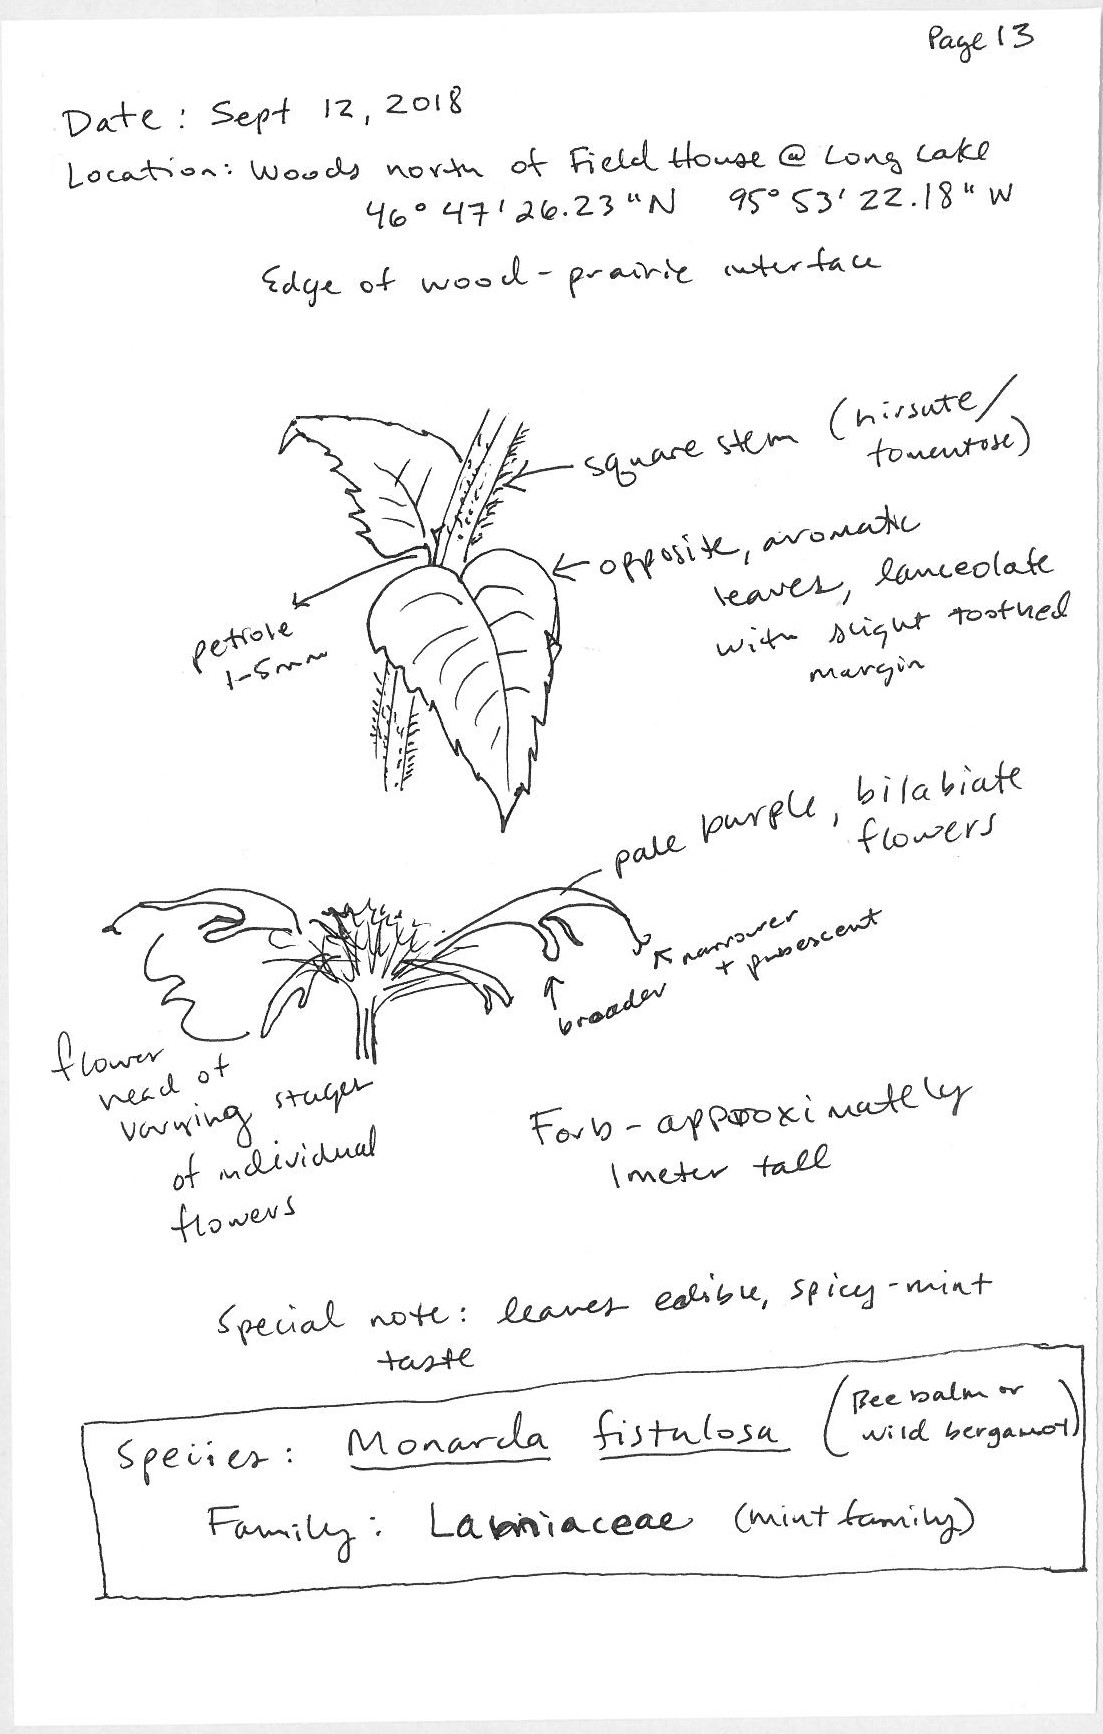
\includegraphics[width=3.8in,angle=90]{example_notebook.jpg}

\newthought{The Family Presentation} will be an oral presentation given in lab on December 5th. Specific guidelines, expectations, and a list of possible families to present on will be handed out at a later date.


\newthought{Participation} in class and lab is essential. Participation is a small part of the final grade; however, a record throughout the semester of exemplary participation and attendance will also help in the case of a borderline final grade. Active participation also nurtures learning, and will improve the quality of future recommendation letters from your instructors.  

\newthought{Extra Credit} will be made available occasionally. One specific way to get extra credit will be to attend the STEM-focused Symposium session, and another will be by participating in a collaboration with a sculpture student. I will provide more details on these opportunities in class.

\subsection{Attendance Policy}

Regular attendance and participation in class is critical to your success at Concordia College. Because any absence, excused or unexcused, detracts from the learning experience, you are expected to attend all classes. Dr.~ArchMiller also values the educational experience afforded by student participation in co-curricular activities; however, you are responsible for notifying Dr.~ArchMiller of scheduled absences (e.g., co-curricular activities) at the beginning of the semester, or as soon as that information is available (but no less than 24 hours in advance). 

If absences become what Dr.~ArchMiller determines to be excessive (from 10-15\% of classes, without valid college-recognized excuses), points will be deducted from your final percentage. In extreme cases ($>20$\% of classes or 6 unexcused absences), Dr.~ArchMiller will assign a failing grade. \textbf{I strongly recommend that you are present and participate in the class.}

%\section{Biology Department Policy on Use of Electronic Devices}

%\begin{enumerate}
%\item All electronic devices (including cellular phones) must be set to silent during scheduled lecture and laboratory sessions.
%\item No electronic devices (laptop computers, PDA, cell phones, MP3 players, digital cameras, etc) should be brought into the classroom during exams, with the exception of materials needed for the exam (e.g., a calculator is permitted if mathematical analysis is required).
%\end{enumerate}






%\newpage

\section{Course Schedule (version dated 8/14/2018)}

\begin{itemize}
	\item This class will be heavily front-loaded because of the waning fall plant season. Thus, we will focus the first month on observing and identifying as many species as possible.
	\item Also, this course counts as a ``field course,'' which means that you must be present in class for at least 24 hours of outdoor field labs (travel to and from field sites does not count). \textbf{It's important to dress appropriately for the weather for all lab sessions.}
	\item Chapters listed are from Murrell \emph{Vascular Plant Taxonomy}

\end{itemize}



  \setlength{\calwidth}{6.5in}
  \setlength{\calboxdepth}{0.55in}
  \begin{calendar}{8/27/18}{17}

  \calday[Monday]{\classday} % Monday
  \calday[Tuesday]{\classday} % Wednesday
  \calday[Wednesday]{\classday}
  \calday[Thursday]{\classday} % Thursday (unnumbered)
  \calday[Friday]{\classday} % Friday
    \skipday\skipday % weekend (no class)

% Week 1
\caltext{8/30/18}{\textbf{First Day of Class}}

% Week 2

\caltext{9/4/18}{Vegetative Terms (Ch 3)}
\caltext{9/5/18}{Field Trip; Hand lens \& Field Notes}
\caltext{9/6/18}{Reproductive Terms (Ch 11)}

% Week 2
\caltext{9/11/18}{\textbf{Terminology Exam}}	
\caltext{9/11/18}{Using keys (Ch 5); Grass \& Aster Terms (p420-425; p492-496)}
\caltext{9/12/18}{Field Trip}
\caltext{9/13/18}{\textbf{Badlands}}
\caltext{9/14/18}{\textbf{Badlands}}

% Week 3
\caltext{9/18/18}{Phylogeny; Scientific \& Common Names (Ch 2, 4, 6)}
\caltext{9/19/18}{\textbf{Symposium} \\ Lab reconvened at Symposium STEM session}
\caltext{9/20/18}{Monilophyta \\ (Ch 9)}

% Week 4
\caltext{9/25/18}{\textbf{Lab Exam 1: Field Notebook Check (15 spp)}}
\caltext{9/26/18}{Field Trip}
\caltext{9/27/18}{Angiosperm Introduction \\(Ch 11)}

% Week 5
\caltext{10/2/18}{Basal Angiosperms \\(Ch 12)}
\caltext{10/3/18}{Field Trip}
\caltext{10/4/18}{Basal Angiosperms \\(Ch 12) cont.}

% Week 6
\caltext{10/9/18}{\textbf{EXAM 1}}
\caltext{10/10/18}{Field Trip}
\caltext{10/11/18}{Monocots \\(Ch 15)}

% Week 7
\caltext{10/16/18}{Monocots \\(Ch 15) cont.}
\caltext{10/17/18}{Field Trip}
\caltext{10/18/18}{\textbf{Lab Exam 2: Field Notebook Check (10 spp)}}


% Week 8
\caltext{10/22/18}{\emph{Mid Semester Break--No Class}}
\caltext{10/23/18}{\emph{Mid Semester Break--No Class}}
\caltext{10/24/18}{\emph{Mid Semester Break--No Class}}
\caltext{10/25/18}{\emph{Mid Semester Break--No Class}}
\caltext{10/26/18}{\emph{Mid Semester Break--No Class}}

% Week 9
\caltext{10/30/18}{Eudicots: Rosids \\(Ch 13)}
\caltext{10/31/18}{Field Trip}
\caltext{11/1/18}{Eudicots: Rosids \\(Ch 13)}

% Week 10

\caltext{11/6/18}{Eudicots: Rosids \\(Ch 13)}
\caltext{11/7/18}{Field Trip}
\caltext{11/8/18}{Eudicots: Asterids \\(Ch 14)}

% Week 11
\caltext{11/13/18}{Eudicots: Asterids \\(Ch 14)}
\caltext{11/14/18}{Field Trip}
\caltext{11/15/18}{Eudicots: Asterids \\(Ch 14)}


% Week 12

\caltext{11/20/18}{\textbf{EXAM 2}}
\caltext{11/21/18}{\emph{Thanksgiving--No Class}}
\caltext{11/22/18}{\emph{Thanksgiving--No Class}}
\caltext{11/23/18}{\emph{Thanksgiving--No Class}}

% Week 13
\caltext{11/27/18}{Gymnosperms \\ (Ch 10)}
\caltext{11/28/18}{Twigs \& Cones lab}
\caltext{11/29/18}{\textbf{Lab Exam 2: Field Notebook Check (5 spp)}}

% Week 14
\caltext{12/4/18}{Gymnosperms \\ (Ch 10)}
\caltext{12/5/18}{Family Presentations}
\caltext{12/6/18}{Gymnosperms \\ (Ch 10)}

% Week 15
\caltext{12/11/18}{Gymnosperms \\ (Ch 10)}
\caltext{12/12/18}{Botany of Food Lab}
\caltext{12/13/18}{Ethnobotany}

% Week 16
\caltext{12/18/18}{\textbf{FINAL EXAM 2:00-4:00pm}}							% change by section


  \end{calendar}



\end{fullwidth}



\newpage

\subsection{Syllabus Acknowledgement}

I, \underline{\hspace{5cm}}, have received a copy of the syllabus for BIOL 221, Ecology, and understand all of the policies and procedures outlined herein. 

\newthought{Signature}  \underline{\hspace{5cm}} {Date}  \hrulefill


\subsection{Use of Photographic Likeness Release}

For good and valuable consideration, I authorize Dr.~ArchMiller to record photographs of me and use, reproduce, modify, distribute, and exhibit such photographs, in whole or in part, without restrictions or limitation for marketing and instructional purposes. 

I release Dr.~ArchMiller, Concordia College, its successors and assigns, agents, and all persons for whom it is acting from any liability by virtue of any blurring, distortion, alteration, optical illusion, or use in composite form, whether intentional or otherwise, that may occur or be produced in the photographic process and waive any right that I may have to inspect or approve the finished recordings.

\newthought{Printed name}  \hrulefill
\newthought{Signature}  \underline{\hspace{5cm}} {Date}  \hrulefill

\subsection{Other Information}

\newthought{Preferred name or nickname} \hrulefill

\newthought{Major} \hrulefill

\newthought{Contact phone number} \hrulefill

\newthought{Where's ``home?''} \hrulefill


\newthought{Why are you taking this class?} \hrulefill

\hrulefill

\hrulefill

\newthought{What are your expectations for this class?}\hrulefill

\hrulefill

\hrulefill
\end{document}                              